\documentclass[aps,pra,notitlepage,amsmath,amssymb,letterpaper,12pt]{revtex4-1}
\usepackage{amsthm}
\usepackage{graphicx}
\usepackage{listings}
\newenvironment{problem}[2][Problem]{\begin{trivlist}
\item[\hskip \labelsep {\bfseries #1}\hskip \labelsep {\bfseries #2.}]}{\end{trivlist}}
\newenvironment{solution}{\begin{proof}[Solution]}{\end{proof}}


\begin{document}

\title{Classwork 13}
\author{Frank Entriken and Grady Lynch}
\affiliation{PHYS 220, Schmid College of Science and Technology, Chapman University}
\date{\today}

\maketitle

\section{Sombrero Potential}

\begin{problem}{Specifications}
Simulate the $x$ and $y$ coordinates of a ball in a double well potential (also known as the "sombrero" potential). Variables to consider are the balls mass, $m$, and the ball's friction as it rolls, $f_{\text{drag}}(\dot{x}) = -\nu \dot{x}$. The "sombrero" will be shaken back and forth repeatedly with a driving force $f_{\text{drive}}(t) = F\cos(\omega t)$.

According to Newton's Second Law, the ball must satisfy the equation of motion: $$m\ddot{x} = f_{\text{hat}}(x) + f_{\text{drag}}(\dot{x}) + f_{\text{drive}}(t) = x - x^3 - \nu \dot{x} + F\cos(\omega t)$$
\end{problem}

\section{The Solution}

\begin{solution}
In order to compute the coordinates of the ball in motion we used the Runge-Kutta 4th Method. This method accurately predicts each subsequent $x$ and $x$ value by considering the approximations before and after the desired value. By using this method we were able to graphically represent the ball's $x$ and $x$ values over the course of its motion. The graphs below represent the ball at different starting values: $x0$ is the starting $x$ position of the ball, $y0$ is the starting $y$ position of the ball, and $F$ which is the force of the shake.

\subsection{Our Graphs}

\begin{figure}[h!]
  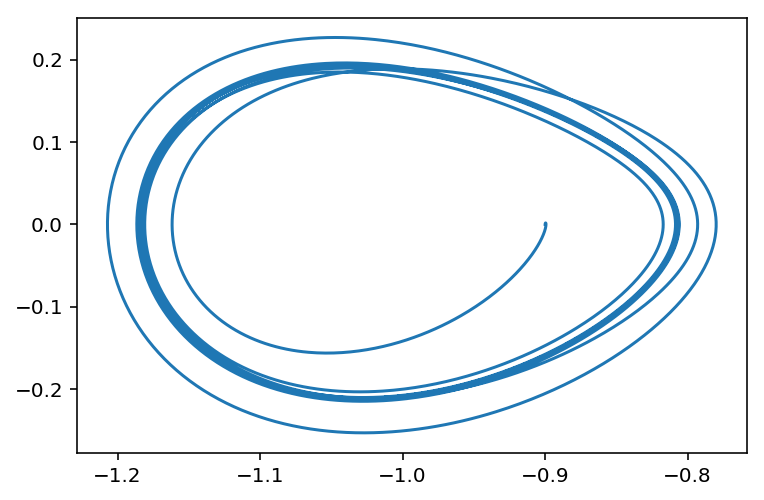
\includegraphics[width=0.4\textwidth]{p1.png}
  \caption{$x0=-0.9$, $y0=0$, $x0=0.18$}
  \label{fig:figlabel}
\end{figure}

\begin{figure}[h!]
  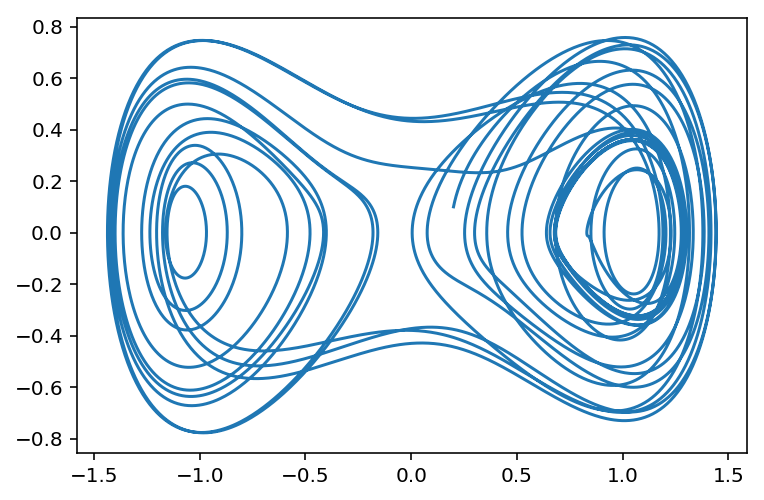
\includegraphics[width=0.4\textwidth]{p2.png}
  \caption{$x0=0.2$, $y0=0.1$, $x0=0.25$}
  \label{fig:figlabel}
\end{figure}

\begin{figure}[h!]
  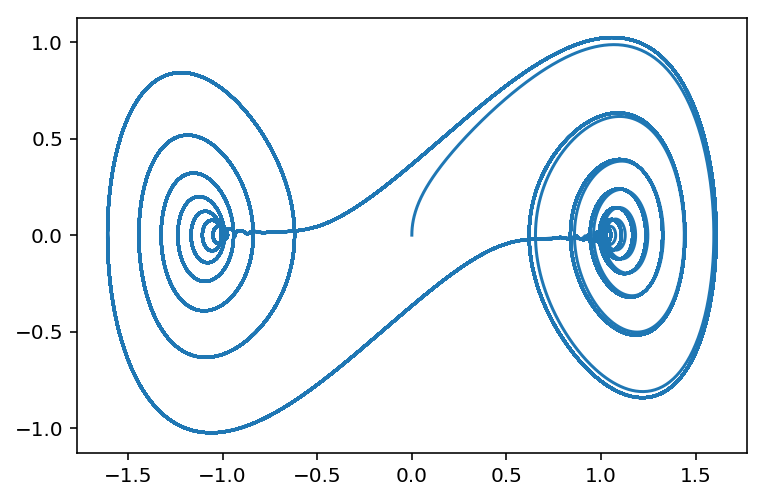
\includegraphics[width=0.4\textwidth]{p3.png}
  \caption{$x0=0$, $y0=0$, $x0=0.4$ \\ The movement of the this graph uses a slightly modified version of the code from $RK4_2$, where our N value is multiplied by a value of 1000 up from 50.}
  \label{fig:figlabel}
\end{figure}


\end{solution}
\end{document}
